\section{Auswertung}
\label{sec:auswertung}
In diesem Kapitel werden die aufgenommenen Messwerte ausgewertet.
\subsection(Der Zerfall von Vanadium)
\label{sec:vanadium}
Die Untergrundstrahlung beläuft sich auf  $13.9 \pm 0.4$ also etwa 14 Zerfälle in einem Zeitintervall
von $\Delta t =\SI{30}{s}$. Diese wurde von der Gemessenen Strahlung abgeszogen anschließend wird
eine Kurve nach \autoref(eq:) an die Messwerte angepasst. Daraus ergeben sich diese Werte für $\lambda$ und 
$N_0$:
\begin{center}
    $ \lambda_V =0.003\pm 0.00$\\
    $N_0=2141.834 \pm 48.628$
\end{center}
Die Anzahl der noch nicht zerfallenen Kerne wird nach \autoref{eq:} beschrieben mit:
\begin{center}
    $N(t)=(2141.834 \pm 48.628) e^{-0.003\frac{1}{s}t}$
\end{center}
Im nachstehenden Plot \autoref{fig:vanadium} sind die Zerfallszahlen ohne Untergrundstrahlung mit zugehörigem 
Fehler nach \autoref{eq:poisson}, die Untergrundstrahlung und das angepasste Zerfallsgesetz dargestellt:
\begin{figure}
    \centering
    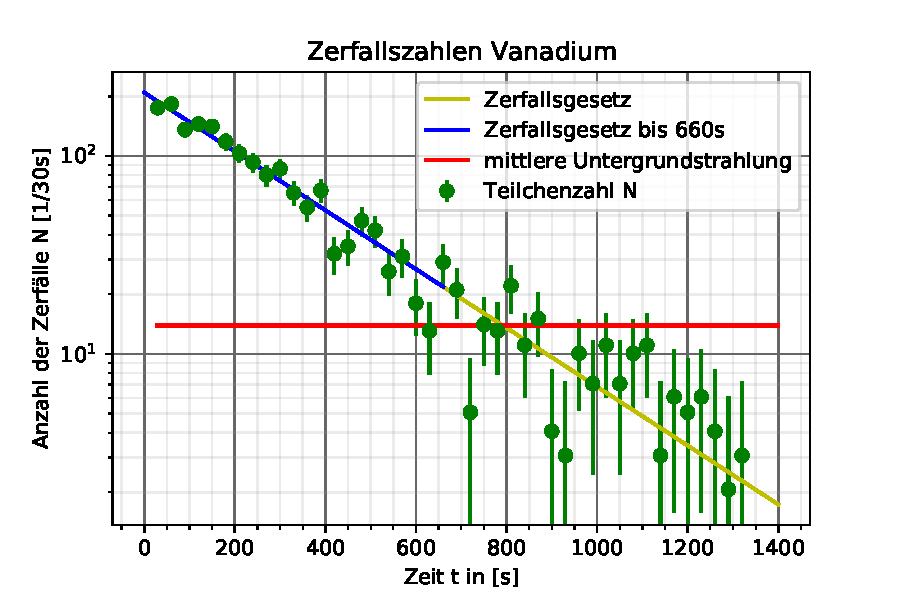
\includegraphics{vanadium.pdf}
    \caption{Zerfall von Vanadium}
    \label{fig:vanadium}
  \end{figure}




\subsection{Der Zerfall von Rhodium}
Die Untergrundstrahlung beläuft sich auf  $6.96 \pm 0.22$ also etwa 7 Zerfälle in einem Zeitintervall
von $\Delta t =\SI{15}{s}$. Diese wird von der gemessenen Gesamtstrahlung subtrahiert und die Ergebniisse
im folgenden Diagramm \autoref{fig:rhodium} mit den nach \autoref{eq:poisson} berechneten Fehlern dargestellt.
Da Rhodium auf zwei arten zerfällt: 
\begin{center} 
    $^{103}_{45}\mathrm{Rh} + \mathrm{n}$ $\rightarrow$ $^{104i}_{45}\mathrm{Rh}$\\
    $^{103}_{45}\mathrm{Rh} + \mathrm{n}$ $\rightarrow$ $^{104}_{45}\mathrm{Rh}$
\end{center}
wird analog zu \autoref{sec:vanadium} zunächst an den bedeutend langsameren Zerfall, der sich anhand der 
Steigungsänderung identifizieren lässt angepasst. Anschließend wird die Anzahl der zerfälle zurückgerechnet und 
von der gesamten Messreihe abgeszogen. Das Resultat ist der Verlauf des schnelleren Zerfalls der in 
\autoref{fig:rhodium1} zu sehen ist. 
  \begin{figure}
    \centering
    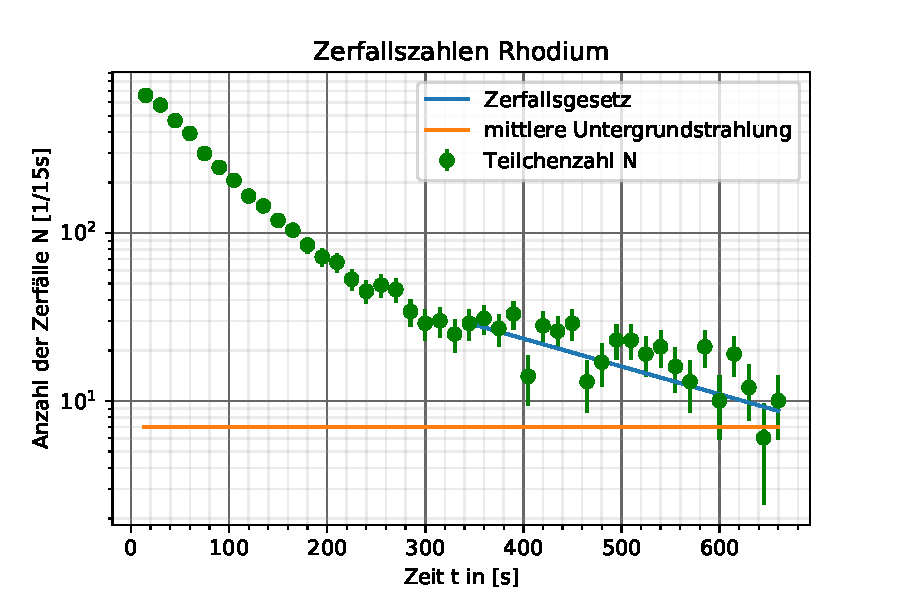
\includegraphics{rhodium.pdf}
    \caption{Zerfall von Rhodium}
    \label{fig:rhodium}
  \end{figure}
An diese \autoref{fig:rhodium1} Messreihe kann dann erneut das Zerfallsgesetz nach \autoref{sec:} angepasst 
werden. 
  \begin{figure}
    \centering
    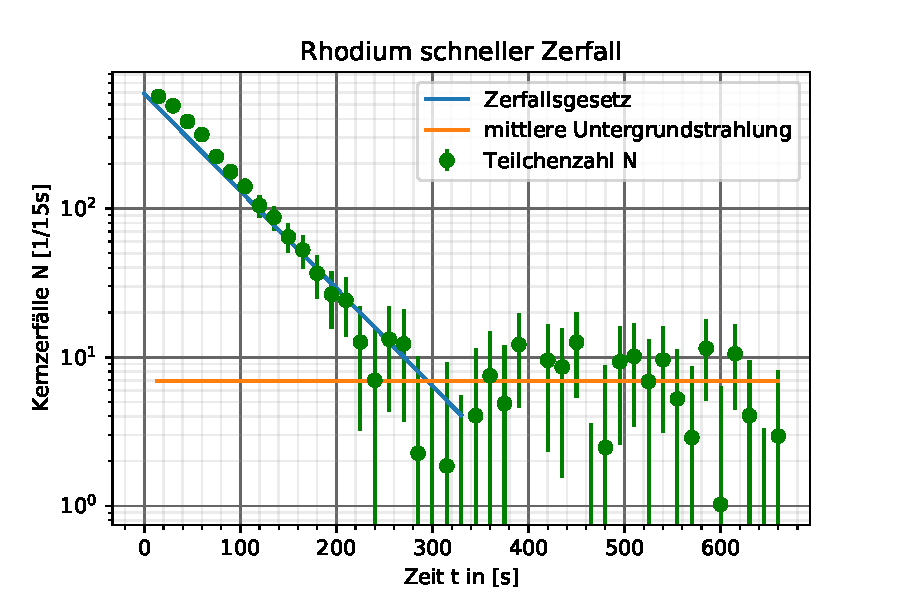
\includegraphics{rhodium1.pdf}
    \caption{Schneller Zerfall von Rhodium}
    \label{fig:magnet}
  \end{figure}
  Es ergibt sich also Zerfallsvorschrift:
  \begin{center}
      $N(t)=N_0 e^{-\lambda t}$
  \end{center}
mit folgenden Werten für den langsameren Zerfall:
\begin{center}
    $\lambda_{Rh1} =0.004\pm 0.001$\\
    $N_{01}=1944.551 \pm 349.657$
\end{center}
und diesen Werten für den schnellen Zerfall:
\begin{center}
    $\lambda_{Rh2} =0.015\pm 0.000$\\
    $N_{02}=2930.865 \pm 48.629$  
\end{center}
